% This must be in the first 5 lines to tell arXiv to use pdfLaTeX, which is strongly recommended.
\pdfoutput=1
% In particular, the hyperref package requires pdfLaTeX in order to break URLs across lines.

\documentclass[11pt]{article}

\usepackage[usenames,dvipsnames]{xcolor}
% Remove the "review" option to generate the final version.
% \usepackage[review]{acl}
\usepackage[]{acl}

% Standard package includes
\usepackage{times}
\usepackage{latexsym}

% For proper rendering and hyphenation of words containing Latin characters (including in bib files)
\usepackage[T1]{fontenc}
% For Vietnamese characters
% \usepackage[T5]{fontenc}
% See https://www.latex-project.org/help/documentation/encguide.pdf for other character sets

% This assumes your files are encoded as UTF8
\usepackage[utf8]{inputenc}

% This is not strictly necessary, and may be commented out,
% but it will improve the layout of the manuscript,
% and will typically save some space.
\usepackage{microtype}

% If the title and author information does not fit in the area allocated, uncomment the following
%
%\setlength\titlebox{<dim>}
%
% and set <dim> to something 5cm or larger.

\title{CLAfICLe: Cross Lingual Adaptation for In-Context Learning}

% Author information can be set in various styles:
% For several authors from the same institution:
% \author{Author 1 \and ... \and Author n \\
%         Address line \\ ... \\ Address line}
% if the names do not fit well on one line use
%         Author 1 \\ {\bf Author 2} \\ ... \\ {\bf Author n} \\
% For authors from different institutions:
% \author{Author 1 \\ Address line \\  ... \\ Address line
%         \And  ... \And
%         Author n \\ Address line \\ ... \\ Address line}
% To start a seperate ``row'' of authors use \AND, as in
% \author{Author 1 \\ Address line \\  ... \\ Address line
%         \AND
%         Author 2 \\ Address line \\ ... \\ Address line \And
%         Author 3 \\ Address line \\ ... \\ Address line}

\author{Giulio Starace \\
  University of Amsterdam / Amsterdam, The Netherlands \\
  \texttt{giulio.starace@gmail.com} \\}

% user settings
\usepackage{graphicx} % for images
\usepackage{subcaption} % for subfigures
\graphicspath{{../figures/}}
\usepackage[export]{adjustbox}
\usepackage{geometry}
\usepackage{booktabs}


\begin{document}
\maketitle
\begin{abstract}
	This document is a supplement to the general instructions for *ACL authors. It contains instructions for using the \LaTeX{} style files for ACL conferences.
	The document itself conforms to its own specifications, and is therefore an example of what your manuscript should look like.
	These instructions should be used both for papers submitted for review and for final versions of accepted papers.
\end{abstract}

\section{Introduction}

Pre-trained large language models (LLMs) are dominating natural language processing (NLP) research
for tackling downstream tasks \citep{devlin_bert_2019,raffel_exploring_2020,brown_language_2020}.
These models rely on the availability of vast amounts of unsupervised training data and the high
usage computing resources that can be leveraged by variants of the transformer architecture
\citep{vaswani_attention_2017}. Because access to such data and compute is limited, and due to the
anglocentric nature of the field, the majority LLM research and application prioritises the English
language. This leads to a large gap between what can be achieved in English and other languages.
Research in multilingual LLMs attempts to address this issue, with encouraging results in many
aspects \citep{conneau_unsupervised_2020,bigscience_workshop_bloom_2022}. These multilingual models
however have been shown to underperform against monolingual counterparts \citep{wu_are_2020}, and
datasets for more niche applications such as fine-tuning for zero-shot and in-context prompted
generalisation remain almost exclusively in English
\citep{bach_promptsource_2022,mishra_cross-task_2022}. One approach to address this issue is
developing techniques for adapting existing English models to work in other languages. Recent
research in model adaptation has shown promising results
\citep{houlsby_parameter-efficient_2019,ainsworth_git_2022}, and there already exist some works
applying these techniques directly to the problem of cross-lingual transfer
\citep{artetxe_cross-lingual_2020}. These works however mainly focus either on encoder-only
transformer (EOT) variants or on performance on a few downstream tasks, through the use of
additional language- and/or task-specific fine-tuning
\citep{de_vries_adapting_2021,gogoulou_cross-lingual_2022}. Works that consider decoder-only
transformer (DOT) variants on the other \citep{de_vries_as_2021, minixhofer_wechsel_2022} limit the
scope to pretrained variants and intrinsic evaluation, with little focus on how their techniques
interact with \textit{fine-tuned} models and their performance on downstream tasks.

This work instead considers techniques for the efficient cross-lingual transfer of models fine-tuned
on \textit{in-context learning} (ICL). Here, the models are fine-tuned to leverage information
presented in the context window to address some downstream task, demonstrating improved performance
and generalisation \citep{wei_finetuned_2021,sanh_multitask_2022,wang_benchmarking_2022}, enabling
multi-task learning and eliminating the need for task-specific fine-tuning. Scaled versions of these
models \citep{chung_scaling_2022} are now on par with the best models from the similarly emerging
paradigm of LLM training with reinforcement learning from human feedback (RLHF)
\citep{ouyang_training_2022}. Lamentably, just like their training, the evaluation of these ICL
fine-tuned models relies on instruction and prompt templates, which are mainly available only in
English. This renders any cross-lingual adaptation of these models futile, as there is no way to
extrinsically evaluate them in the target language. Recent work from \citet{min_metaicl_2022}
circumvents this requirement by directly fine-tuning a model on chains of input-output pairs from
a suite of tasks, matching the performance of instruction-based ICL. We therefore focus on adapting
models trained under this particular framework, and present the following contributions:
\begin{enumerate}
	\item We show that \citet{minixhofer_wechsel_2022}'s WECHSEL language-adaptation technique scales,
	      successfully adapting the large variant of GPT2 (774M) to French and German. We release the our
	      checkpoints, which previously did not exist at this parameter scale for these languages.
	\item We continue the evaluation of WECHSEL by measuring its robustness by applying it to
	      a fine-tuned variant of GPT2 and measuring its performance on a number of downstream tasks,
	      rather than just examining perplexity.
	\item We share our methods and results for adapting fine-tuned models capable of ICL from English to
	      French and German.
	\item We introduce the notion of ``targeted distillation'', a form of post-hoc disentanglement
	      leveraging adapters \citep{houlsby_parameter-efficient_2019} to extract only the fine-tuned
	      information from a fine-tuned model.  We refer to our technique as \textsc{PHoDiVA}
	      (\textbf{P}ost \textbf{Ho}c \textbf{Di}sentanglement via \textbf{V}essel \textbf{A}dapters).
\end{enumerate}

\section{Related Work}

todo

\section{Methods and Models}\label{sec:method}

\subsection{MetaICL}

Due to the complete lack of prompting/instruction templates in non-English languages, we rely on
MetaICL \citep{min_metaicl_2022}, which circumvents the need for prompt/instruction templates at
train-time and test-time. With MetaICL, a pretrained DOT is fine-tuned by concatenating $k$ examples
of input-output pairs (``shots'') from a variety of tasks and feeding this as input to the model.
The final input-output pair is truncated such that only the input is shown, and the model is trained
to predict the output using a negative log-likelihood objective from a number of possible options.
The trained model is then generalises to unseen tasks presented in the same way by utilizing the $k$
shots provided in the context.  We refer to this model as \textit{MetaICL}.

\subsection{Sandwich}

As a baseline, we consider the obvious solution of simply translating input in the target language
to English, feeding the translation to MetaICL, and translating the output back to the target
language. We refer to this model as \textit{Sandwich}. We make use of Google's Cloud Translation AI
API\footnote{\href{https://cloud.google.com/translate}{https://cloud.google.com/translate}}.

\subsection{WECHSEL}

Aside from translation API calls, to adapt a monolingual DOT from a source language to a target
language we employ WECHSEL \citep{minixhofer_wechsel_2022}, which has shown success in adapting the
small variant of GPT2 (117M parameters) to a number of target languages. WECHSEL works by retraining
the tokenizer into the target language and re-initializing the transformer embedding layers such
that the target embeddings are semantically similar to the source embeddings. This is done by
leveraging existing parallel multilingual static word embeddings. As done by
\citet{de_vries_adapting_2021}, after re-initialization, additional causal language modeling (CLM)
is performed in the target language to account for syntactical differences. Applying WECHSEL to
MetaICL, we obtain what we refer to as \textit{MetaICL-geWECHSELt}.

\subsection{Adapters}\label{sec:method:adapters}

Because we are interested in adapting a fine-tuned DOT (MetaICL), we hypothesize that the additional
CLM at the end of WECHSEL can lead to catastrophic forgetting of the fine-tuning. Furthermore, we
hypothesize that the fine-tuning may contain language-specific information, entangled with the task
information relevant to the fine-tuning objective. To address this issue, inspired by MAD-X
\citep{pfeiffer_mad-x_2020} we train a ``task adapter'' on the same ICL objective and data as
MetaICL with a GPT2 base, obtaining an ``ICL-adapter'', which we refer to as \textit{MetaICLA}.
Adapters introduce ``bottleneck'' dense layers at each transformer layer of their base. The adapter
is trained on a particular objective while the base is kept frozen, allowing for parameter-efficient
and modular fine-tuning. These dense layers consist in a down matrix $\mathbf{W}_{down}$, projecting
the hidden states into a lower dimension $d_{bottleneck}$, a non-linearity $f$, which is applied to
this projection and an up matrix $\mathbf{W}_{up}$ that projects back to the original dimension:
\begin{equation} \mathbf{h} \leftarrow \mathbf{W}_{up} f(\mathbf{W}_{down} \mathbf{h}) + \mathbf{r},
\end{equation} where $r$ is a residual connection. Having separated the task-specific information,
we apply WECHSEL to the GPT2 base, obtaining what we refer to as \textit{GPT2-geWECHSELt}. Adding
MetaICLA to GPT2-geWECHSELt, we obtain a model theoretically capable of ICL in the target language,
\textit{GPT2-geWECHSELt+MetaICLA}.

\subsection{\textsc{PHoDiVA}}

To address situations where repeating fine-tuning is not permissible, either because the data is not
released, the process too complicated or the compute simply not available, we propose
\textsc{PHoDiVA}. Here, instead of repeating ICL fine-tuning, we leverage the fine-tuned MetaICL
checkpoint, using it as a teacher in a modified student-teacher offline distillation
\citep{hinton_distilling_2015} setup. More specifically, before WECHSEL adaptation, we add
a ``vessel'' adapter to a (frozen) GPT2 base, and then perform CLM in the source language (English).
Vessel adapters are exactly the same as task adapters, except that they act as a ``vessel'' for
distilled capabilities rather than as additional parameters for fine-tuning. Rather than predicting
the actual next word, the adapter is trained to predict the next word greedily sampled from the
teacher. The idea is to overfit the adapter to the teacher outputs (hence the greedy sampling).
Because the GPT2 base is frozen and theoretically shares the original language modeling capabilities
of the teacher, we hypothesize that this ``targeted distillation'' can disentangle the fine-tuned
capabilities into the vessel adapter. We use the CLM objective because of the constraint to keep the
distillation process as simple as possible, so to make it advantageous over repeating a potentially
complex fine-tuning process. The only constraint of this method is that the adapter base is the same
pretrained base that was fine-tuned into the teacher. When using MetaICL as the teacher, we refer to
the resulting vessel adapter as \textit{MetaICLVA}. Like in section \ref{sec:method:adapters}, after
applying WECHSEL to a GPT2 base, we can then combine the language-adapted base and MetaICLVA to
obtain \textit{GPT2-geWECHSELt+MetaICLVA}, another model theoretically capable of ICL in the target
language.

\section{Experimental Setup}

We use the PyTorch Lightning Python framework \citep{falcon_pytorch_2019} to implement our work.
Because we envision the direct application of this work to be most useful to smaller companies and
start-ups, we limit our compute to a single 40GB NVIDIA A100 GPU and run jobs for a maximum of 24
hours. Our code is available on
GitHub\footnote{\href{https://github.com/thesofakillers/CLAfICLe}{https://github.com/thesofakillers/CLAfICLe}}.

\subsection{Models}

There exist various possible adapter setups, specifying different configurations of the up and down
weight matrices, non-linearity and residual connection, among other settings. For our work, we use
the \verb_pfeiffer_ configuration from AdapterHub \citep{pfeiffer_adapterhub_2020}.

Regarding MetaICL, \citet{min_metaicl_2022} train a number of variants, releasing checkpoints
however only for variants fine tuning the large version of GPT2 (774M parameters). We base the rest
of our models on the same GPT2 version and use the ``high resource to low resource'' direct MetaICL
checkpoint as we consider this to be the most realistic. We make use of the HuggingFace Transformers
\citep{wolf_transformers_2020} implementation of GPT2 throughout.

\subsection{Evaluation}

For assessing ICL, we reimplement the same evaluation setup as \citet{min_metaicl_2022}, evaluating
a given model on a suite of tasks, prepending the input with $k=16$ training examples sampled
randomly for each task. For our evaluation metrics, like \citet{min_metaicl_2022}, we use F1 for
tasks where the label options change across examples, and accuracy for tasks where the label options
are always the same. Because the evaluation benchmark used by \citet{min_metaicl_2022} is limited to
English, we develop our own multilingual multi-task benchmark spanning 9 different tasks across
3 languages (English, German, and French). Our benchmark design is restricted to tasks that can be
handled by the MetaICL framework, namely multi-class, single-label tasks. To enable complete
comparisons across languages, we also restrict our benchmark to only contain language-parallel
datasets. Correspondingly, we list the ICL benchmark datasets in Table \ref{tab:benchmark}.

\begingroup
\setlength{\tabcolsep}{0.5pt}
% Please add the following required packages to your document preamble:
% \usepackage{booktabs}
\begin{table}[t]
	\centering
	\caption{The datasets constituting our ICL benchmark. Most originate from pre-existing benchmarks,
		namely XGLUE \citep{liang_xglue_2020} and \citep{lin_common_2021}.}
	\label{tab:benchmark}
	\begin{tabular}{@{}llc@{}}
		\toprule
		\multicolumn{1}{l}{Dataset} & \multicolumn{1}{l}{(Origin)}    & Collection \\ \midrule
		HateCheck                   & \citep{rottger_hatecheck_2021}  & -          \\
		XNLI                        & \citep{conneau_xnli_2018}       & XGLUE      \\
		QAM                         & \citep{liang_xglue_2020}        & XGLUE      \\
		QADSM                       & \citep{liang_xglue_2020}        & XGLUE      \\
		PAWS-X                      & \citep{yang_paws-x_2019}        & XGLUE      \\
		MARC                        & \citep{keung_multilingual_2020} & -          \\
		X-CODAH                     & \citep{lin_common_2021}         & XCSR       \\
		X-CSQA                      & \citep{lin_common_2021}         & XCSR       \\
		Wino-X                      & \citep{emelin_wino-x_2021}      & -          \\ \bottomrule
	\end{tabular}
\end{table}
\endgroup

To evaluate the successful application of WECHSEL to GPT2, we use the same process as
\citet{minixhofer_wechsel_2022}, namely measuring perplexity on a held out test set. For all
language modeling, we use the original release of the OSCAR corpus
\citep{ortiz_suarez_monolingual_2020}.

\subsection{Training}

When performing CLM training, due to our limited compute, we heed the advice of
\citet{geiping_cramming_2022} and pack as samples into 1024-token sequences (the maximum length
possible) by separating them with EOS tokens, so to minimize the number of padding tokens and
maximize GPU utilisation. With this we are able to fit a batch size of 2 into memory, while actually
presenting the model with more than two examples per batch in most cases\footnote{This technique is
	also suggested by HuggingFace in their CLM tutorial:
	\href{https://huggingface.co/course/chapter7/6}{https://huggingface.co/course/chapter7/6}.}. We
achieve a virtual batch size of 512 by accumulating gradients over 256 steps. We employ single-epoch
training \citep{komatsuzaki_one_2019} on a total of 600M tokens, which we estimate to be the number
of tokens consumed by our model in a single epoch by running a profiling run on a smaller download.
Based on the information in \citet{geiping_cramming_2022} and \citet{minixhofer_wechsel_2022}, we
decide to use Adam \citep{kingma_adam_2015} with a linear warmup for the first half of training to
a peak learning rate of 5e-4, followed by cosine annealing to 0 by the end of training. When
performing targeted distillation for MetaICLVA, we reduce the linear warmup to the first 10\% of
training to help with our voluntary overfitting. As suggested by \citet{izsak_how_2021}, to maximize
training time, we evaluate on only 0.5\% of the data, logging every 50 steps.

For the ICL training necessary for MetaICLA, we modify \citet{min_metaicl_2022}'s implementation so
to work with adapters. In particular, we use their \verb+HR→LR+ training mixture, which consists of
61 tasks sourced from the \textsc{CrossFit} \citep{ye_crossfit_2021} and \textsc{UnifiedQA}
\citep{khashabi_unifiedqa_2020} benchmarks.

\section{Results and Discussion}
\begin{figure}[t]
	\centering
	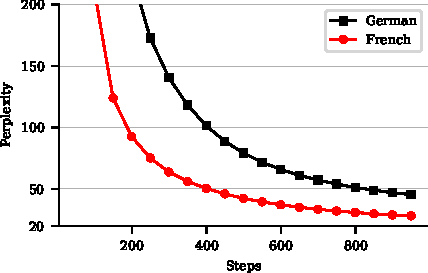
\includegraphics{gpt2-w_ppl.pdf}
	\caption{Perplexity on the held out set when performing the recommended CLM training after WECHSEL
		language-adaptation of GPT2. A step corresponds to an optimizer update. We evaluate every 50
		steps.}
	\label{fig:gpt2-w_ppl}
\end{figure}

Fig.\@ \ref{fig:gpt2-w_ppl} shows the performance of GPT2 after around 1k steps of training,
evaluated intrinsically in terms of perplexity. For both French and German, we see perplexity
decrease to sub-50 values, with the French model reaching a perplexity of $\approx$ 28. Both models
are clearly underfit, still monotonically decreasing by the end of the training. These observations
are roughly in-line with \citet{minixhofer_wechsel_2022}'s findings for smaller variants of GPT2,
although we train for much less time and hence are left with higher perplexities. While we believe
our preliminary results suggest WECHSEL scales well to larger models in terms of intrinsic
evaluation, future work may wish to investigate whether this holds for longer training times. The
rest of our work considers, among other questions, the robustness of WECHSEL via extrinsic
evaluation on downstream tasks performed by MetaICL.

\begin{figure*}[ht]
	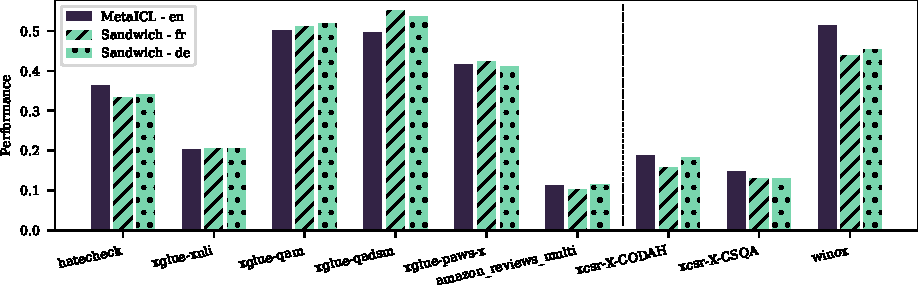
\includegraphics{baselines.pdf}
	\caption{Performance (max is 1) on a particular language dimension of our multi-task benchmark of
		our two baseline models, MetaICL and Sandwich. The dashed line separates whether a given task uses
		accuracy (left) or F1-score (right) as the performance metric.}
	\label{fig:baselines}
\end{figure*}

Fig.\@ \ref{fig:baselines} shows the performance on each dataset of our benchmark for the two
baseline models, MetaICL and Sandwich. As summarized in Table \ref{tab:results-summary}, Sandwich
performs roughly on par with MetaICL on both target languages, respectively with scores of 0.317 and
0.322 in French and German compared to MetaICL's score of 0.327 in English. We note generally low
scores across all tasks. This is particularly perplexing in the case of MetaICL, scoring around
0.1 points less than with the evaluation ensemble used by \citet{min_metaicl_2022}, where the same
checkpoint was reported scoring 0.417 in the worst case (a 25 \% decrease). While similar values
are reached in certain tasks in our benchmark (e.g. most of XGLUE and WINO-X), it is unclear what
the origin of this discrepancy is, whether due to differences in evaluation implementation or
difficulty of the tasks. Given that \citet{min_metaicl_2022} simply report macro-averaged scores,
it is impossible to verify the latter. Nevertheless, our results suggest that Sandwich-like
solutions may be satisfactory for transferring performance from English to other languages given
the surprisingly closeness of the scores. The decision between using Sandwich or ``properly''
adapted models with the same capabilities then becomes an economic one in terms of the cost of API
calls (for the former) versus the cost of inference plus training (for the latter).

\begin{figure*}[ht]
	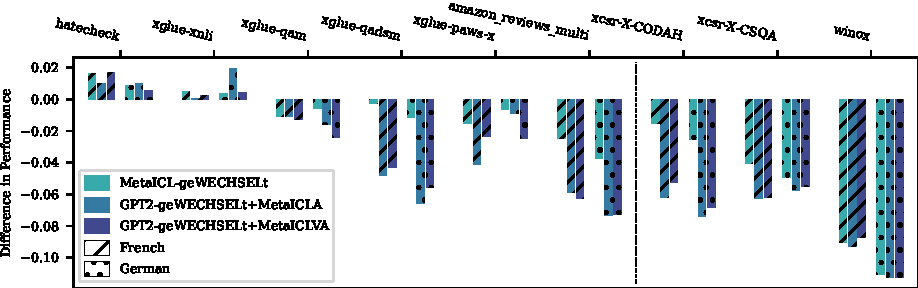
\includegraphics{results.pdf}
	\caption{Performance gap on our multi-task benchmark between each of the language-adapted models
		and the ``Sandwich'' baseline. Positive values indicate that the adapted models are
		outperforming the baseline, while negative values indicate the reverse. The dashed line
		separates whether a given task uses accuracy (left) or F1-score (right) as the performance
		metric.}
	\label{fig:results}
\end{figure*}

Fig.\@ \ref{fig:results} shows the difference in performance on each dataset of our benchmark
between the proposed models and Sandwich. In general, we observe that the proposed models
underperform across almost all tasks in both French and German, with the trends aligning at
a task-level (e.g. all models underperform on QAM, by roughly the same amount). As reported in Table
\ref{tab:results-summary}, the best of our proposed models is MetaICL-geWECHSELt, which
underperformed Sandwich by roughly 0.02-0.03 points. This undermines the motivation for the other
two models, which were designed to avoid catastrophic forgetting by separating language and ICL
capabilities via adapters. The results suggest that the tradeoff between catastrophic forgetting and
needing to train ICL-adapters leans in favour of the former in this compute regime. In this sense,
we can conclude that WECHSEL does not suffer tremendously due to catastrophic forgetting when
adapting fine-tuned DOTs such as the MetaICL variant of GPT2.

Our work is mainly limited by its preliminary nature. Apart for considering more appropriate
(\textit{sc.} larger) compute scales, future work could investigate training ICL-adapters more
thoroughly, for example by performing hyperparameter optimization or incorporating more recent
adapter research such as AdapterDrop \citep{ruckle_adapterdrop_2021}, AdapterFusion
\citep{pfeiffer_adapterfusion_2021} or Hyper-X \citep{ustun_hyper-x_2022}.

We are also interested in a more complete treatment of \textsc{PHoDiVA}. For instance, future work
could explore different forms of student-teacher distillation, consider other forms of loss
criterions, use beam search rather than greedy sampling and/or take inspiration from similar
solutions such as \citet{khrulkov_disentangled_2021}'s work on generative models. We believe work in
this direction could benefit from simplifying the problem setting first, by considering a smaller,
encoder-only transformer fine-tuned on a single downstream task on a single-language.

Other future work may consider different adaptation approaches that have recently emerged. For
example, \citet{marchisio_mini-model_2022}'s Mini-Model adaptation has yet to be tested on
decoder-only transformers, and it would be interesting to see how it compares to WECHSEL in this
regard. Other, slightly more distant approaches such as meta-learning a-la X-MAML
\citep{nooralahzadeh_zero-shot_2020} may provide different results.

Perhaps a clear limitation of this direction of research is that the setting remains monolingual.
Future work could explore whether it is possible to adapt a monolingual model to multiple languages
simultaneously, and how such adaptations would compare to monolingual-to-monolingual adaptation in
terms of resources and performance. Finally, undermining all of this work is our restriction to
results on a single random seed. Future work with more seeds and more compute would be necessary to
draw more definitive conclusions.

\begin{itemize}
	\item TODO: few datasets, lack of multilingual data, problem with datasets being machine
	      translated
	\item consider other general fine-tuning paradigms such as RLHF
\end{itemize}

\begin{table}[ht]
	\centering
	\caption{Average performance (max is 1) across the datasets from our multi-task benchmark for the
		models considered in this work. We use ``W'' as a shorthand for ``geWECHSELt''. We report average
		difference in performance for each proposed alternative to Sandwich. Negative values indicate
		underperformance compared to Sandwich.}
	\label{tab:results-summary}
	\begin{tabular}{@{}rccc@{}}
		\toprule
		\multicolumn{1}{c}{} & en    & fr     & de                             \\ \midrule
		MetaICL              & 0.327 & -      & -                              \\
		Sandwich             & -     & 0.317  & 0.322                          \\ \midrule
		\multicolumn{4}{c}{\textit{Difference in Performance w.r.t. Sandwich}} \\
		MetaICL-W            & -     & -0.020 & -0.026                         \\
		GPT2-W+MetaICLA      & -     & -0.041 & -0.042                         \\
		GPT2-W+MetaICLVA     & -     & -0.036 & -0.045                         \\ \bottomrule
	\end{tabular}
\end{table}

\section{Conclusion}

We explore the problem of language-adapting a monolingual DOT previously fine-tuned to perform
in-context learning. To this end, we stress test the current SoTA adaptation method, WECHSEL,
scaling to previously untested model sizes, applying it a fine-tuned variant of GPT2 (MetaICL) and
evaluating extrinsically on a multi-task benchmark. While we find that WECHSEL successfully scales
to larger model sizes, we find that at our compute regime, WECHSEL-adapted MetaICL underperforms
compared to simply sandwiching the English model between translation API calls. We experiment with
separating ICL fine-tuning and language adaptation to address potential catastrophic forgetting
through the use of Adapters, but find these approaches unsuccessful. In doing so, we propose
\textsc{PHoDiVA}, a novel method for post-hoc disentanglement through vessel adapters. We share
\textsc{PHoDiVA} in this rudimentary form as a starting point for future work in this direction.

\bibliography{anthology,custom}

\section{Appendices}

Use \verb|\appendix| before any appendix section to switch the section numbering over to letters.
See Appendix~\ref{sec:appendix} for an example.

\appendix
\section{Example Appendix}
\label{sec:appendix}

This is an appendix.

\end{document}
